% UTF-8 encoding
% Compile with latex+dvipdfmx, pdflatex, xelatex or lualatex
% pdflatex is recommanded
% This template is released under BSD 2-Clause license.
\documentclass[UTF8]{ctexart}
%====================================================
% 颜色和自定义颜色
\usepackage{xcolor}
\definecolor{hyperref-green}{RGB}{0,150,0}
\definecolor{hyperref-red}{RGB}{200,0,0}
\definecolor{hyperref-blue}{RGB}{0,0,200}
%====================================================

%====================================================
% 超链接
\usepackage[
pagebackref=true,
citecolor=hyperref-blue,
linkcolor=hyperref-blue,
urlcolor=hyperref-green,
menucolor=black,
letterpaper=true,
breaklinks=true,
bookmarks=true,
colorlinks
]{hyperref}
\usepackage{bibentry}
%====================================================

%====================================================
%导入外部pdf
\usepackage{pdfpages} % includepdf
%====================================================

%====================================================
% 公式和数学标识,算法流程图
\usepackage{amsmath}
\usepackage{bm} %%某些矢量需要加粗字符,除mathbf外的另一种方式%By Kuber
\usepackage{amssymb}
\usepackage{pifont}
\usepackage{listings} %插入代码

\let\counterwithout\relax
\let\counterwithin\relax
\usepackage[ruled]{algorithm2e} %算法和伪代码
\newcommand{\cmark}{\checkmark}%
\newcommand{\xmark}{\ding{55}}%
\usepackage{xcolor} % math color
\usepackage{diagbox}
\numberwithin{equation}{section} % 公式按章节编号
\numberwithin{table}{section} % 公式按章节编号
% 声明argmin和argmax运算符
\newcommand{\argmin}{\mathop{\mathrm{argmin}}\limits}
\newcommand{\argmax}{\mathop{\mathrm{argmax}}\limits}
\usepackage{amsfonts}
%====================================================

%====================================================
% 插入图表和图表描述
\usepackage{graphicx, caption, subfigure, float}
\DeclareCaptionFormat{myformat}{\fontsize{8}{8}\selectfont#1#2#3}
\captionsetup{format=myformat}
\captionsetup{margin=2cm}
\captionsetup{justification=centering}
\usepackage{overpic}
% 绘图
\usepackage{pgfplots}
%====================================================

%====================================================
% 其他格式,和样式
% 将章节标号转为中文
\usepackage{zhnumber}  
%% geometry
\usepackage{geometry}
\geometry{left=3.17cm,right=3.17cm,top=3.0cm,bottom=3.0cm}  % 页边距
% 页眉相关的设置
\usepackage{fancyhdr}
\fancyhf{}  % 清除默认页眉
\pagestyle{fancy}
\lhead{上海大学硕士学位论文}  % 添加右侧页眉
\rhead{KAI ZHAO: \url{http://kaiz.xyz}}  % 右侧页眉,写你自己的论文的时候请去掉本行。
\cfoot{\thepage}  % 添加页脚页码
%% 设置章节格式
\CTEXsetup[name={第, 章}]{section}
\CTEXsetup[number={\chinese{section}}]{section}
\CTEXsetup[format+={\zihao{-2}}]{section}   % 大章节字体: 小二
\CTEXsetup[beforeskip={17pt}]{section} % 标题与上面文本的间距%By Kuber
\CTEXsetup[afterskip={16.5pt}]{section}  % 标题与下面文本的间距%By Kuber
\CTEXsetup[format+={\zihao{3}}]{subsection} % 小章节字体: 三号
\CTEXsetup[beforeskip={13pt}]{subsection}%同上,间距可调
\CTEXsetup[afterskip={13pt}]{subsection}%同上,间距可调
\CTEXsetup[beforeskip={13pt}]{subsubsection}%同上,间距可调
\CTEXsetup[afterskip={13pt}]{subsubsection}%同上,间距可调
\CTEXsetup[format+={\zihao{3}}]{subsection} % 小章节字体: 三号
\CTEXsetup[format+={\zihao{-4}}]{subsubsection}
% 图表按章节编号
\usepackage{chngcntr}
\counterwithin{figure}{section}
%====================================================

%====================================================
%常用的命令
\newcommand{\red}[1]{{\textcolor{red}{#1}}}%
%====================================================

%====================================================
% 开始正文
\begin{document}
\zihao{-4} %
\linespread{1.6} \selectfont  % 调整全文为1.6倍line间距,非常接近word版本1.5行间距%By Kuber

% 导入封面内容,注意这个地方的页码请根据你的实际情况设置,
% 我的cover.pdf有6页,所以是插入1-6页

\includepdf[pages={1-7}]{cover.pdf} 
\pagenumbering{Roman} % 目录之前的内容(包括目录)页码使用罗马数字
\setcounter{page}{7}  % LaTeX的起始页码
%%%%%%%%%%%%%%%%%%%%%%%%%%%%%%%%%%%%%%%%%%%%%%%%%%%%%%%%%%%%%
% 此处请大家务必注意!!
% 由于本人能力/精力有限,并没有设计毕业论文‘目录之前的所有内容’
% 包括‘封面,中/英文摘要,原创说明,授权说明’等内容,
% 这些版面的设计也并非LaTeX的长处。
% 因此这部分需要你使用cover.docx编写,然后导出cover.pdf,
% 最后在LaTeX中·includepdf[1-X]{cover.pdf}。
% 注意,上面的页码请根据你得到的pdf的实际页码填写。
% 还需注意,为了让word的页码和LaTex的页码连续(LaTex页码默认从1开始),
% 需要为LaTex手动设置起始页码:
% \setcounter{page}{X}  % LaTeX的起始页码
% 这里的X要根据你自己的cover.docx页数而定。
%%%%%%%%%%%%%%%%%%%%%%%%%%%%%%%%%%%%%%%%%%%%%%%%%%%%%%%%%%%%%

% 由于目录(TOC: table of contents)也会被hyperref作为超链接,因此颜色会被设置为和图表超链接一样的红色,红色的目录不好看。
% 这里单独把TOC的颜色设置为黑色。
{\hypersetup{linkcolor=black}
\tableofcontents}

\pagebreak
\section{绪论}
\pagenumbering{arabic} % 正文开始,页码使用阿拉伯数字
\setcounter{page}{1}
\subsection{关于\LaTeX模板}
这个\LaTeX是我为了写学位论文而写的,本项目的主页为 \url{http://kaiz.xyz/shu-thesis},
代码都host在\href{https://github.com/zeakey/shu-thesis}{Github}。
%
虽然这个模板写的很简陋,但是完成学位论文写作应该是够用了。

\subsection{关于\TeX和\LaTeX}
\href{https://en.wikipedia.org/wiki/TeX}{\TeX}是由图灵奖得主,程序(program)和算法(algorithm)这两个概念的
提出者,《计算机程序设计的艺术》(The Art of Computer Programming)的作者,著名计算机科学家
Donald E. Knuth(高德纳)发明的排版系统。TeX是特别优秀的排版工具,尤其善于处理复杂的图表和公式。
%
\href{https://en.wikipedia.org/wiki/LaTeX}{\LaTeX}(拉泰赫)是一种基于\TeX的排版系统,由由美国计算机学家Leslie Lamport(莱斯利·兰伯特)在20世纪80年代初期开发,
因此被称为Lamport Tex,简称LaTeX。

\subsection{使用哪个\LaTeX发行版}
\LaTeX拥有众多的发行版,主要有一下几个:
\begin{table}[!h]
  \centering
  %\renewcommand{\arraystretch}{1}
  \setlength\tabcolsep{6.4pt}
  \begin{tabular}{c|c|c|c}
    \hline
    \diagbox{发行版}{支持平台} & Windows & Linux & OSX \\
    \hline
    \href{http://www.tug.org/texlive/}{TexLive} & \cmark  & \cmark &  \cmark \\
    \hline
    \href{https://miktex.org/}{MikTex} & \cmark  & \xmark & \xmark  \\
    \hline
    \href{http://www.tug.org/mactex/}{MacTex} & \xmark  & \xmark & \cmark  \\ \hline
    \end{tabular}\vspace{-6pt}
  \caption{主要的\LaTeX发行版。
  }\label{tab:latex-distr}%
\end{table}%
我比较推荐TexLive,因为它支持主流的平台,而且更新频率也比较高。

\subsection{使用哪个\TeX编辑器}
市面上的\TeX编辑器也是五花八门,选择一个合适的编辑器会让你事半功倍。
我常用的编辑器是\href{http://www.xm1math.net/texmaker/}{TexMaker},
支持双栏预览,左边代码右边预览。
当然也有很多其他的选择,比如Windows平台上比较常用的\href{http://www.winedt.com/}{WinEdit}。
Vim用户还可以使用\href{https://github.com/lervag/vimtex}{VimTex}插件。

\paragraph{在线编辑环境}现在有很多以\url{https://overleaf.com}为代表的
在线的\LaTeX写作平台。
%
这些在线平台普遍支持\red{多人协作}并内置了很多学术期刊会议的模板,而且编译环境在远端
因此\red{不用配置本地环境和安装编辑器}。
%
但由于是在线平台,储存空间有限,而且不能编译太大的源文件
(比如overleaf不支持编译50+pages的文档)。
%
而且由于众所周知的原因,在中国大陆访问这些网站有些时候会出现一些问题。

%%%%%%%%%%%%%%%%%%%%%%%%%%%%%%%%%%%%%%%%%%%%%%%%%%%%%%%
\section{公式}
%%%%%%%%%%%%%%%%%%%%%%%%%%%%%%%%%%%%%%%%%%%%%%%%%%%%%%%
方便快捷的公式输入是\LaTeX相比于Word的主要优势之一,在熟练掌握的情况下
公式输入的效率会有很大提升。

\LaTeX中的公式主要分为两类:\red{行内公式}和\red{行间公式}。
这是一个行内公式$f(x) = \frac{1}{\sqrt{2\pi}\sigma}\exp{(-\frac{(x-\mu)^2}{2\sigma^2})}$。下面是一个行间公式:
$$
f(x) = \frac{1}{\sqrt{2\pi}\sigma}\exp{(-\frac{(x-\mu)^2}{2\sigma^2})}
$$
这是一个带有编号的公式:
\begin{equation}
f(x)= |x| = 
\begin{cases}
x,& \text{if } x\geq 0\\
-x,              & \text{otherwise}
\end{cases}
\label{eq:cases}
\end{equation}
多行连等公式:
\begin{equation}
\begin{split}
f(x) &= |x| \\
&= \begin{cases}
x,& \text{if } x\geq 0\\
-x,              & \text{otherwise}
\end{cases}
\end{split}
\end{equation}
带有矩阵的公式:
\begin{equation}
\mathbf{H} = -\mathbf\mu \cdot \mathbf{B} = -\gamma B_o \mathbf{S}_z = -\frac{\gamma B_o\hbar}{2} 
\begin{bmatrix}
1& \cdots &1\\ 
\vdots & \ddots & \vdots \\
1 & \cdots & 1 
\end{bmatrix}.
\label{eq:matrix}
\end{equation}
带有矢量的公式:%By Kuber
\begin{equation}
\label{eq:current_density_inandout}
\bm{J_i} = -\sigma_i \nabla \phi_i ~;~ \bm{J_e}= -\sigma_e \nabla \phi_e ~.
\end{equation}
带有联立大括号的公式:%By Kuber
\begin{equation}
\label{eq:runge_p_eq}
\left\lbrace
\begin{aligned}
V_{i+1} &= V_i + c_1 K_1 + c_2 K_2 + \cdots + c_p K_p \\
K_1 &= \Delta t f(t_i ,V_i) \\
K_2 &= \Delta t f\left(t_i + a_2 \Delta t, V_i + b_{21} K_1\right) \\
\cdots&~\cdots~\cdots~\cdots~\cdots~\cdots \\
K_p &= \Delta t f\left( t_i + a_p \Delta t, V_i + b_{p1} K_1 + \cdots + b_{p,p-1} K_{p-1}\right) ~.
\end{aligned}
\right.
\end{equation}
对于一个神经网络的求解问题可以公式化成以下形式:
\begin{equation}
\Theta = \argmin_{\theta} J(\theta)
\label{eq:argmin}
\end{equation}
式\ref{eq:argmin}中$\Theta$为求得的最佳参数,$\theta$为神经网络的参数,$J(\theta)$为误差函数。

公式可以添加label属性,并在后文中引用。比如公式~\ref{eq:matrix}就可以被引用,
而且点击引用号可以迅速跳转,详情请见第\ref{sec:ref}章。

%%%%%%%%%%%%%%%%%%%%%%%%%%%%%%%%%%%%%%%%%%%%%%%%%%%%%%%
\section{算法和伪代码}
%%%%%%%%%%%%%%%%%%%%%%%%%%%%%%%%%%%%%%%%%%%%%%%%%%%%%%%
有时候我们需要在论文中插入一些代码片段来详细说明算法的步骤,
或者需要插入一个伪代码片段来说明算法的流程。

\subsection{插入代码}
% 设置代码样式(关键词颜色,背景颜色,插入代码语言等等)
\lstdefinestyle{customc}{
  belowcaptionskip=1\baselineskip,
  breaklines=true,
  frame=L,
  xleftmargin=\parindent,
  language=C,
  showstringspaces=false,
  basicstyle=\footnotesize\ttfamily,
  keywordstyle=\bfseries\color{green!40!black},
  commentstyle=\itshape\color{purple!40!black},
  identifierstyle=\color{blue},
  stringstyle=\color{orange},
  numbers=left,
}
\lstdefinestyle{customasm}{
  belowcaptionskip=1\baselineskip,
  frame=L,
  xleftmargin=\parindent,
  language=[x86masm]Assembler,
  basicstyle=\footnotesize\ttfamily,
  commentstyle=\itshape\color{purple!40!black},
}
% 插入c语言代码
\lstset{escapechar=@,style=customc}

\begin{lstlisting}[caption={一段C语言程序。},captionpos=b]
#include <stdio.h>
#define N 10
/* Block
 * comment */

int main()
{
    int i;

    // Line comment.
    puts("Hello world!");
    
    for (i = 0; i < N; i++)
    {
        puts("LaTeX is also great for programmers!");
    }

    return 0;
}
\end{lstlisting}

\begin{lstlisting}[caption={一段Python语言程序。},captionpos=b,language=Python]
from mpl_toolkits.mplot3d import Axes3D
import matplotlib.pyplot as plt
import numpy as np
fig = plt.figure()
ax = fig.add_subplot(111, projection='3d')
for c, z in zip(['r', 'g', 'b', 'y'], [30, 20, 10, 0]):
    xs = np.arange(20)
    ys = np.random.rand(20)
    # You can provide either a single color or an array. To demonstrate this,
    # the first bar of each set will be colored cyan.
    cs = [c] * len(xs)
    cs[0] = 'c'
    ax.bar(xs, ys, zs=z, zdir='y', color=cs, alpha=0.8)
ax.set_xlabel('X')
ax.set_ylabel('Y')
ax.set_zlabel('Z')
plt.show()
fig.savefig('bar3d.pdf')
\end{lstlisting}

\subsection{插入伪代码}
\begin{algorithm}[H]
\SetAlgoLined
\KwResult{Write here the result }
 initialization\;
 \While{While condition}{
  instructions\;
  \eIf{condition}{
   instructions1\;
   instructions2\;
   }{
   instructions3\;
  }
 }
 \caption{一个简单的算法。}
\end{algorithm}
%%%%%%%%%%%%%%%%%%%%%%%%%%%%%%%%%%%%%%%%%%%%%%%%%%%%%%%
\section{图表}
%%%%%%%%%%%%%%%%%%%%%%%%%%%%%%%%%%%%%%%%%%%%%%%%%%%%%%%
\subsection{插入图片}
\LaTeX支持多种格式的图片,其中包括png、jpg等常见位图,以及pdf、eps等\textbf{矢量图}格式。
矢量图尤其适合科技论文中用于数据展示的各种曲线图和柱状图、饼状图,因为无论如何缩放图像都不会失真。你可以尝试缩放生成的pdf文件到最大,然后观察图~\ref{fig1},图~\ref{fig3}和图\ref{fig:fig3d}中的曲线。

\begin{figure}[!h]
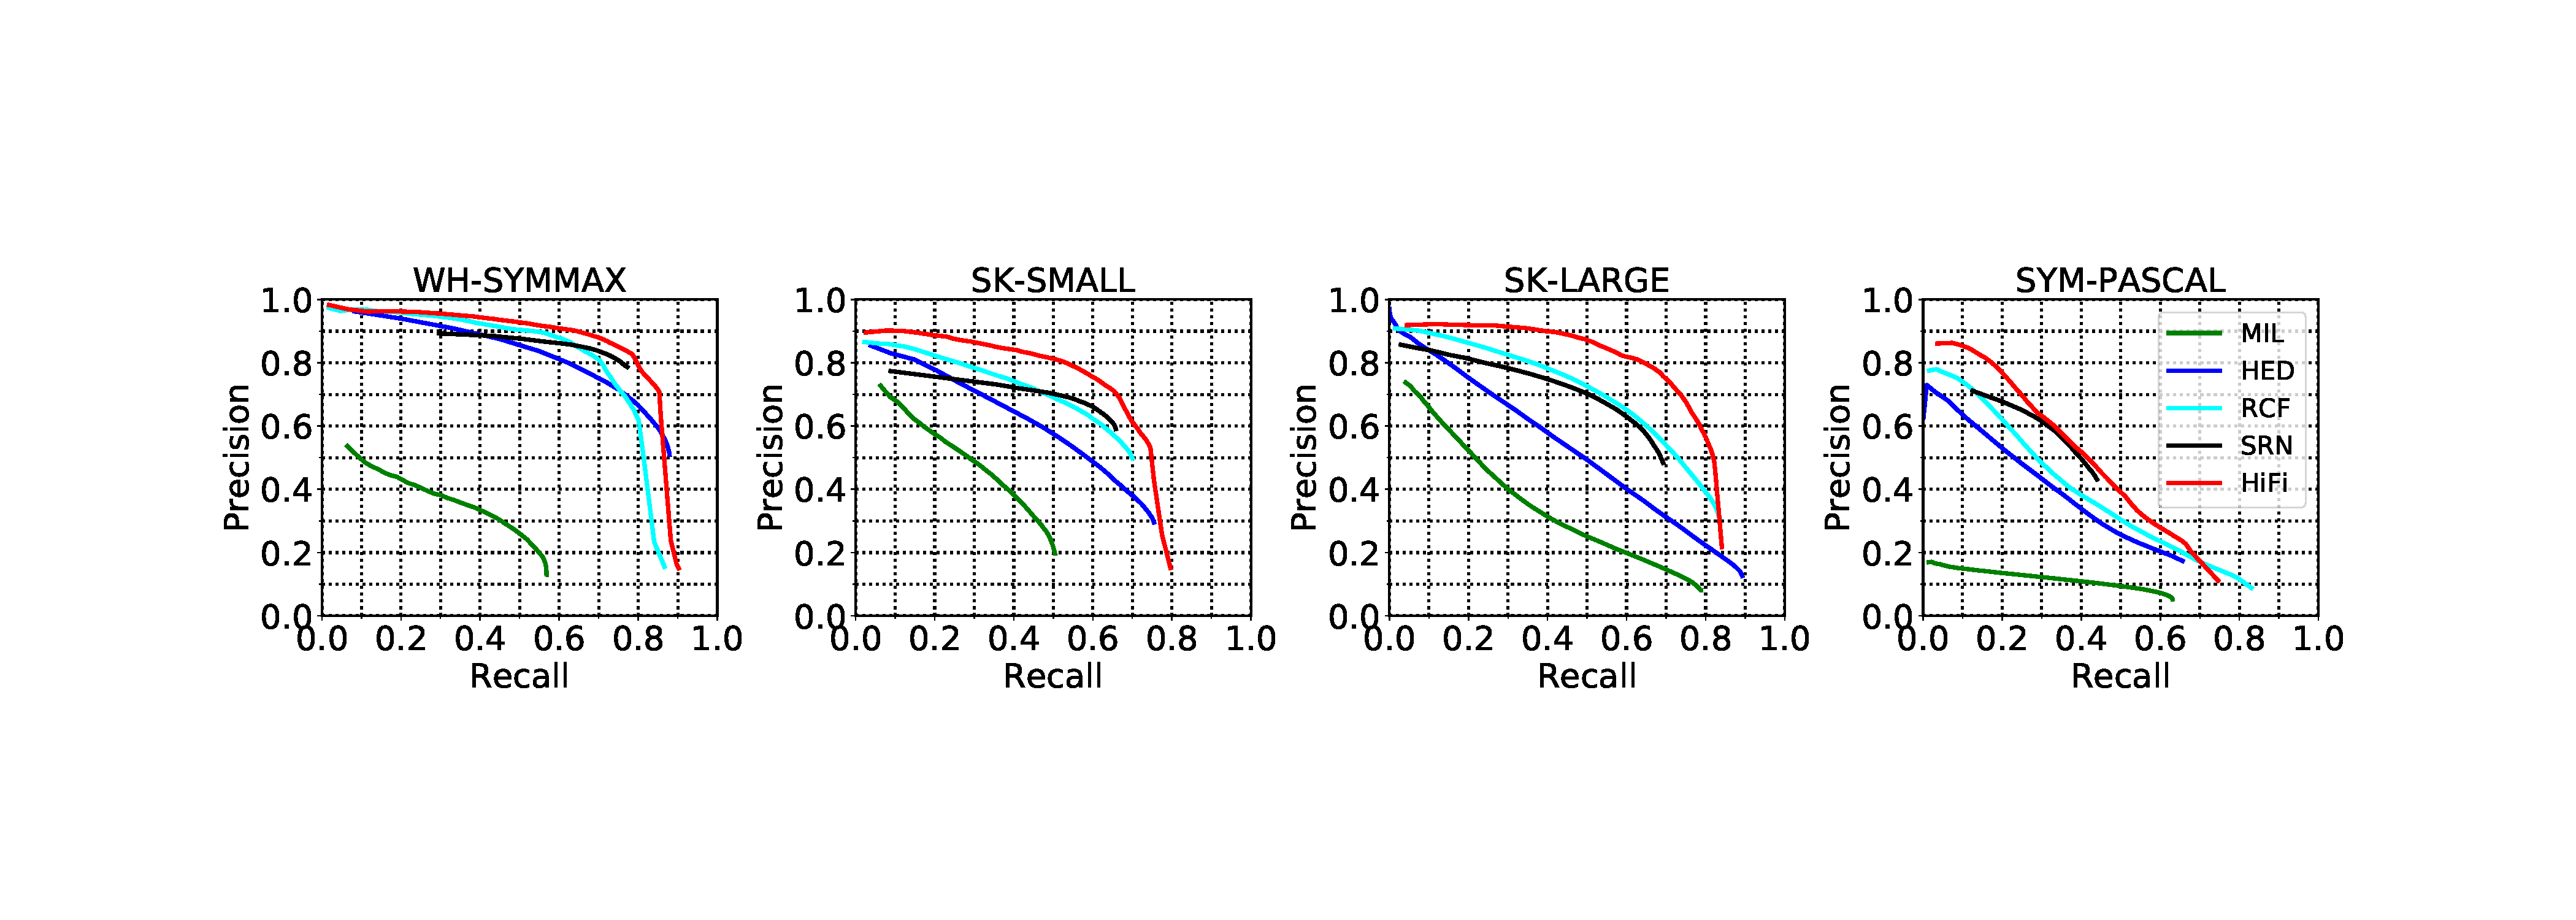
\includegraphics[width=1\linewidth]{figures/pr-curve}
\caption{一个pdf格式的矢量图。使用\\caption命令为图表添加注解,注解中可以引用参考文献~\cite{shen2017label}。}\label{fig1}
\end{figure}

对于曲线图和柱状图等非照片类图表,我推荐插入pdf格式。pdf格式支持绝大部分主流平台(Windows, Linux, OSX),而且可以方便的自由编辑,文件大小也比较小。
如果你使用Python的Matplotlib画图,那么可以直接用matplotlib.pyplot.savefig()
来导出.pdf格式的图片。
如果你使用Matlab画图的话,只能导出eps格式的矢量图。在\LaTeX中插入eps也没有问题,
但是eps文件比同等条件的pdf稍大,而且不方便编辑。
强迫症患者可以将eps转为pdf后再插入到\LaTeX。

同样是一行四列的布局,图~\ref{fig1}直接插入一个包含四个曲线图的pdf文件,
而图~\ref{fig:fig3d}通过增加一个$1\times4$的表格,然后再每个表格单元中各自插入
一个图标文件。

\begin{figure}[!h]
\centering
\begin{overpic}[scale=0.6]{figures/convergence}
\put(50,41){\large{可使用overpic命令}}
\put(38, 35){\Large{往图像上覆盖符号$\Sigma$}}
\put(35,28){\LARGE{公式$f(x)=a\times x$}}
\put(30,20){\huge{引用公式\ref{eq:cases}。}}
\put(25,12){\Huge{参考文献\cite{shen2016object}。}}
\end{overpic}
\caption{一个pdf格式的矢量图。使用\\caption命令为图表添加注解,注解中可以引用参考文献~\cite{shen2017deepskeleton}。}
\label{fig3}
\end{figure}

\begin{figure}[!h]
\centering
  \begin{tabular}{@{}cccc@{}}
    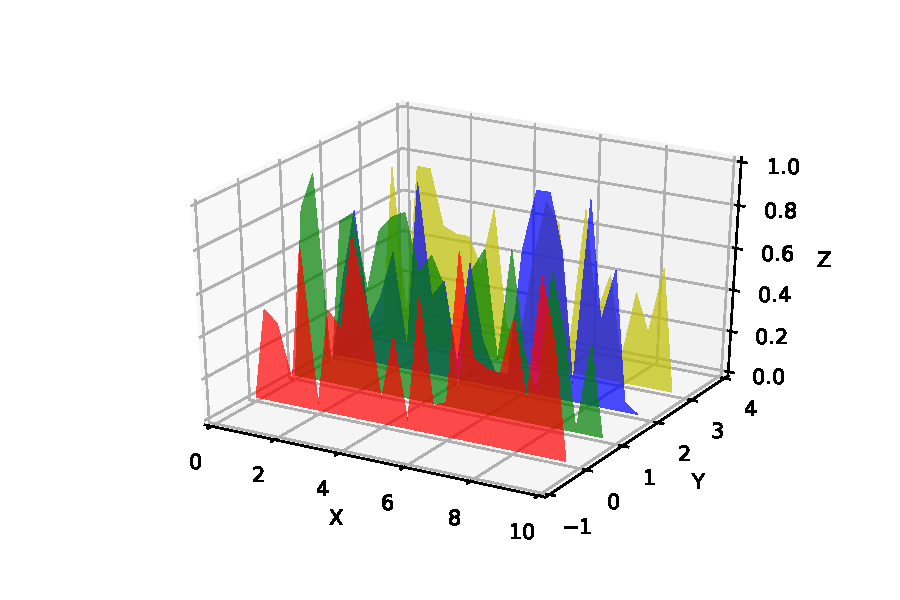
\includegraphics[width=.25\textwidth]{figures/mplot3d}  &
    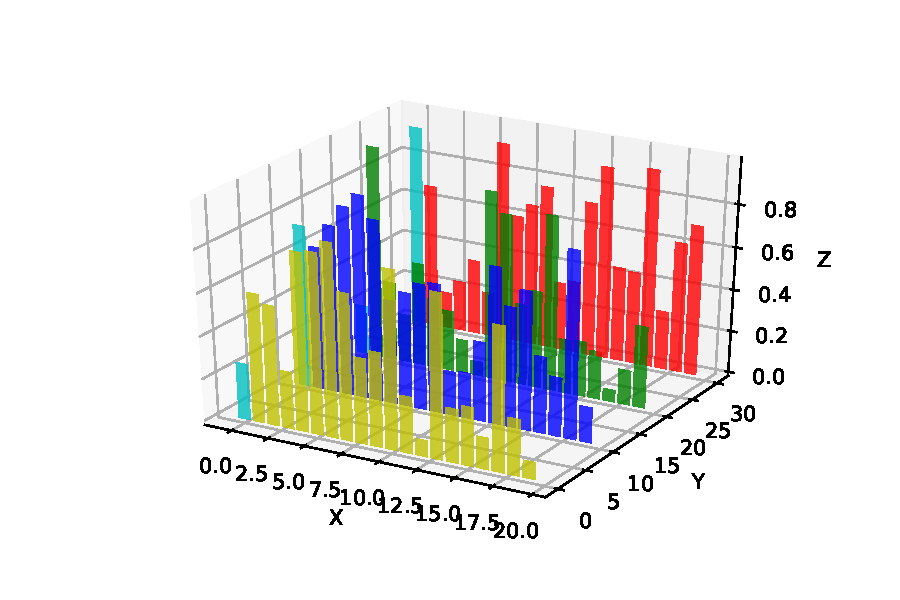
\includegraphics[width=.25\textwidth]{figures/bar3d}  &
    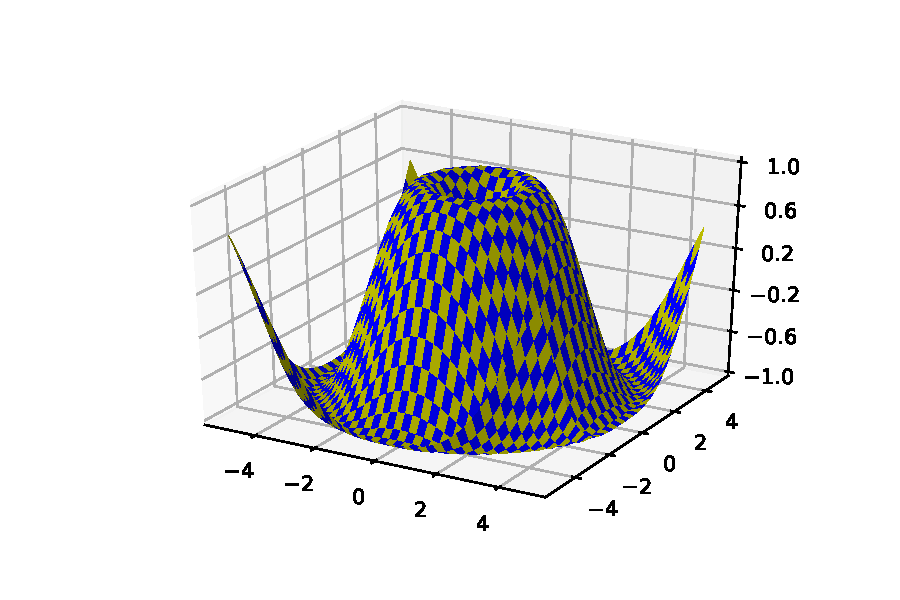
\includegraphics[width=.25\textwidth]{figures/surface3d} &
    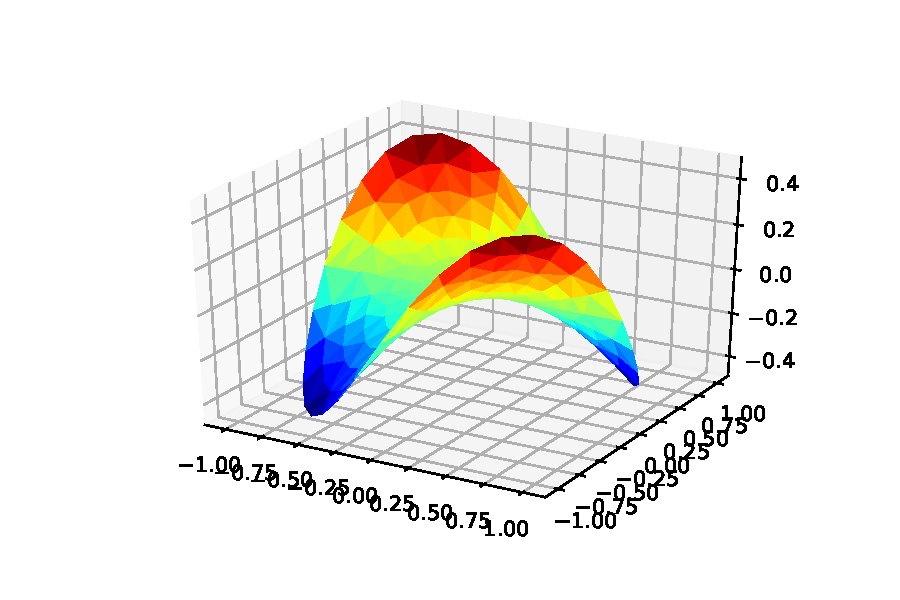
\includegraphics[width=.25\textwidth]{figures/trisurf3d} \\
    (a)M-plot 3D & (b)Bar-chart 3D & 
    (c)Surface 3D & (d) Tri-surface 3D \\
  \end{tabular}
  \caption{通过表格对图片进行布局,在一个$1\times4$表格的每一个单元格中各自插入一个图片文件。
  生成上面四个图对应的Python代码在\href{https://github.com/zeakey/shu-thesis/tree/master/figures}{figures}目录下。}
  \label{fig:fig3d}
\end{figure}
下面是相关代码:
\begin{lstlisting}[captionpos=b,language=Tex]
\begin{figure}[!h]
\centering
  \begin{tabular}{@{}cccc@{}}
    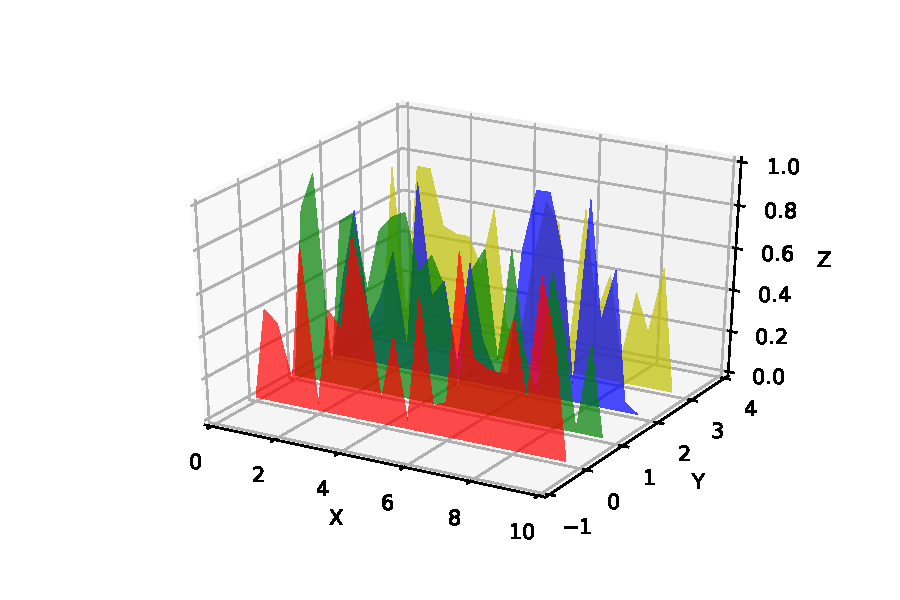
\includegraphics[width=.25\textwidth]{figures/mplot3d}  &
    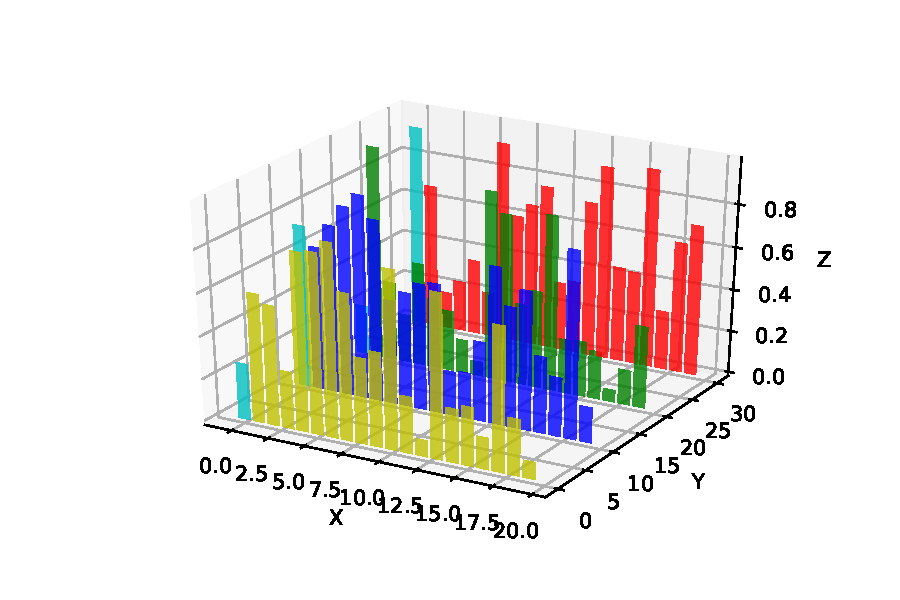
\includegraphics[width=.25\textwidth]{figures/bar3d}  &
    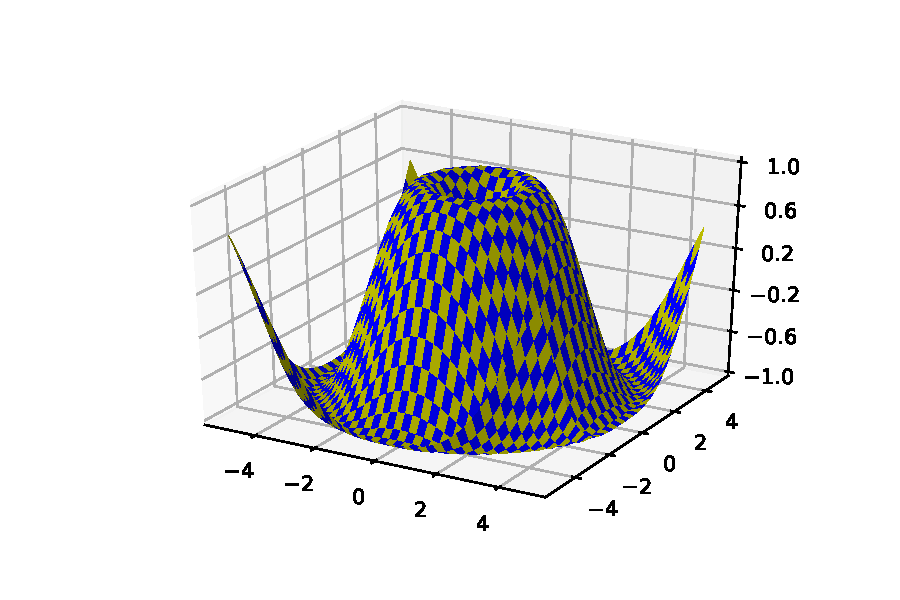
\includegraphics[width=.25\textwidth]{figures/surface3d} &
    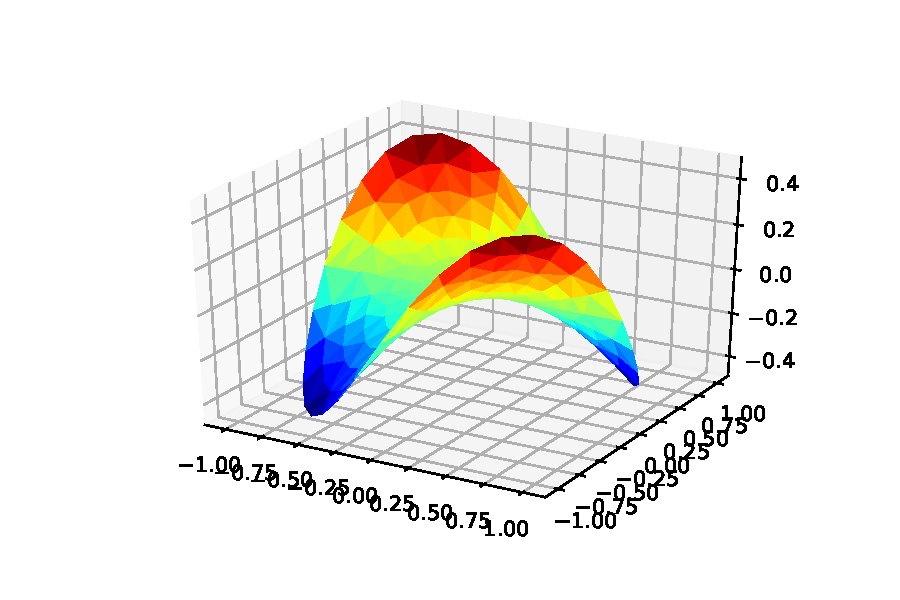
\includegraphics[width=.25\textwidth]{figures/trisurf3d} \\
    (a)M-plot 3D & (b)Bar-chart 3D & 
    (c)Surface 3D & (d) Tri-surface 3D \\
  \end{tabular}
\end{figure}
\end{lstlisting}

\subsection{绘图}
除了通过直接插入已经生成的图像文件之外,\LaTeX 还可以通过 Tikz 宏包直接绘制函数图像。
%
下面有几个使用Tikz包绘制三位函数曲面和直方图的例子,由于 Tikz 会让编译的时间变长,代码已经被注释。
%
如果你有兴趣的话可以取消注释然后编译查看效果,或者预览预编译的pdf:
\url{http://data.kaiz.xyz/shu-thesis/shu-thesis.pdf}。

%\begin{figure}[!h]
%\centering
%\begin{tabular}{@{}cc@{}}
%  \pgfplotsset{width=0.5\textwidth}
%  \begin{tikzpicture}
%    \begin{axis}[
%    hide axis,                              %隐藏坐标
%    colormap/cool,                          %颜色风格
%    ]
%    \addplot3[
%    mesh,                                   %绘制的三维图像是网格
%    samples=50,                             %定义域分割数量
%    domain=-8:8,                            %定义域
%    ]
%    {sin(deg(sqrt(x^2+y^2)))/sqrt(x^2+y^2)};    %二元显式函数
%        \addlegendentry{$\frac{sin(r)}{r}$}         %添加图例
%    \end{axis}
%  \end{tikzpicture} & 
%  %==============================%
%  \pgfplotsset{width=0.5\textwidth}
%  \begin{tikzpicture}
%    \begin{axis}[colorbar]         % 绘制坐标,并设置一个彩色指示条
%    \addplot3[surf]                % 绘制三维图
%    {x^2+y^2};                    % 输入二元显式函数
%    \end{axis}
%  \end{tikzpicture}
%\end{tabular}
%\caption{通过Tikz绘制函数图像。}
%\label{fig:tikz_surface}
%\end{figure}
%还有直方图:
%\begin{figure}[!hbt]
%\centering
%\pgfplotsset{width=0.5\textwidth}
%\begin{tikzpicture}
%\begin{axis}[ybar,enlargelimits=0.15]  % 绘制关于y坐标的条形图,条形之间的最大间隔是0.15cm
%\addplot[draw=blue,fill=red]           % 蓝色边界、红色填充
%coordinates
%{
% (0,4) (1,1) (2,2)
% (3,5) (4,6) (5,1)
%};
%\addplot[draw=black,fill=blue]         % 黑色边界、蓝色填充
%coordinates
%{
% (0,3) (1,4) (2,2)
% (3,9) (4,6) (5,2)
%};
%\end{axis}
%\end{tikzpicture}
%\caption{通过Tikz绘制直方图。}\label{fig:tikz_hist}
%\end{figure}
%

本章节的所有图像都是\textbf{使用\LaTeX 代码直接绘制的},并没有使用任何Matlab或者matplotlib等第三方程序生成图像。
当然,生成的的图像全部都是矢量图。

%\pagebreak
\subsection{表格}
\LaTeX使用table环境生成表格。下面就是生成表\ref{tab:performance}的\LaTeX代码:

\begin{lstlisting}[captionpos=b,language=Tex]
\begin{table}[!h]
  \centering
  \setlength\tabcolsep{6.4pt}
  \begin{tabular}{l|c|c|c|c}
    \hline
    \diagbox{Method}{Dataset} & A & B & C & D \\
    \hline
    LMSDS~\cite{shen2017deepskeleton} & 0.365  & 0.392 & 0.293 & 0.174 \\
    LDLF~\cite{shen2017label} & 0.732  & 0.542 & 0.497 & 0.369 \\
    \hline
    \textbf{FSDS} (ours) & 0.769  & 0.623 & 0.633 & 0.418 \\
    \hline
    \end{tabular}\vspace{-6pt}
  \caption{This is a table.}\label{tab:sk-fmeasure}\label{tab:performance}%
\end{table}%
\end{lstlisting}

\begin{table}[!h]
  \centering
  \setlength\tabcolsep{6.4pt}
  \begin{tabular}{l|c|c|c|c}
    \hline
    \diagbox{Method}{Dataset} & A & B & C & D \\
    \hline
    LMSDS~\cite{shen2017deepskeleton} & 0.365  & 0.392 & 0.293 & 0.174 \\
    LDLF~\cite{shen2017label} & 0.732  & 0.542 & 0.497 & 0.369 \\
    \hline
    \textbf{FSDS} (ours) & 0.769  & 0.623 & 0.633 & 0.418 \\
    \hline
    \end{tabular}\vspace{-6pt}
  \caption{This is a table.}\label{tab:sk-fmeasure}\label{tab:performance}%
\end{table}%

\subsection{图表的排版和定位}\label{sec:location}
\LaTeX相比Word有个缺点就是\emph{非所见即所得}。比如你的两个表格在代码中明明是
相邻一个在前一个在后的,然而排版出来的结果可能是两个被放到了不同的页面中,甚至先后顺序都不对应。
%

\LaTeX图表使用位置参数来确定元素的定位。位置参数有以下几种选项:h (here)、t (top)、b (bottom)、p (我也不知道),分别表示把元素至于当前位置、当前页面的上方、下方。
当你有排版困惑,怎么弄也无法把图标放在自己想要的位置的时候(我经常遇到),最好的解决方法就是疯狂前后移动图表元素对应代码,总有一个位置会是对的。
%
\href{https://tex.stackexchange.com/questions/35125/how-to-use-the-placement-options-t-h-with-figures}{这里}是一个对位置参数的详细介绍。

%%%%%%%%%%%%%%%%%%%%%%%%%%%%%%%%%%%%%%%%%%%%%%%%%%%%%%%
\section{交叉引用}\label{sec:ref}
%%%%%%%%%%%%%%%%%%%%%%%%%%%%%%%%%%%%%%%%%%%%%%%%%%%%%%%
交叉引用可以说是\LaTeX的核心竞争力了。
我们经常需要在论文中引用文献和文章中的图表,比如说:“根据文献
~\cite{shen2017label},~\cite{shen2016object}和~\cite{shen2017deepskeleton}
所描述的的方法,
以式\ref{eq:cases}作为评价标准,我们可以得到如图~\ref{fig1}所示的性能曲线以及
表~\ref{tab:sk-fmeasure}中的定量型能比较。从图~\ref{fig1}和表~\ref{tab:sk-fmeasure}的结果来看,~\cite{shen2016object}和~\cite{shen2017deepskeleton}
具有较好的检测效果”。

如果你使用Word撰写学位论文,可以想象一下情景:你的论文有50+条引用,
你要在论文中反复交叉引用这些参考文献;然后现在你发现你的绪论部分需要补充一条
参考文献,而有的引用格式要求参考文献引用标号按文中出现先后的顺序排列,
当插入一条参考文献之后你如何处理后续的参考文献编号?
%%


或者有下面一个场景:当你完成第三章写作之后发现图3.6和图3.7之间要再插入一张图,然后
你发现图3.7和图3.7之后的所有图片的标号都要改,而且你的文中所有引用到这些图的地方都需要修改。

\textbf{\LaTeX强大的交叉引用功能}将把你从繁琐的文献/图表/公式标号中解放出来,
你只用关注写作本身,其他的事情会帮你自动完成。
%
当你写完一个图表/公式,给它添加一个label属性,然后在需要引用的地方使用ref\{the-label\}
进行引用,\LaTeX将自动为你排好序号。
%
比如"根据文献~\cite{shen2017label},~\cite{shen2016object}
和~\cite{shen2017deepskeleton}所描述的的方法,
以式\ref{eq:matrix}作为评价标准,我们可以得到如图~\ref{fig1}所示的性能曲线以及
表~\ref{tab:sk-fmeasure}中的定量型能比较。从图~\ref{fig1}和表~\ref{tab:sk-fmeasure}的结果来看,~\cite{shen2016object}和~\cite{shen2017deepskeleton}
具有较好的检测效果"。

\TeX文档中的所有内容都可以添加label属性从而进行交叉引用。比如说文章的一个子章节
(subsection)就可以被引用:第\ref{sec:location}章描述了如何对\TeX元素进行定位。

更强大的是,所有的生成的引用标号都是可以点击的,
当你在生成的pdf中点击引用标号,将自动弹到对应的文献/图表/公式处。
%
另外,在文章最后的参考文献列表中,每一条参考文献的末尾都会标注这条参考文献在哪一页被引用。

%


%%%%%%%%%%%%%%%%%%%%%%%%%%%%%%%%%%%%%%%%%%%%%%%%%%%%%%%
\section{有用的链接}
%%%%%%%%%%%%%%%%%%%%%%%%%%%%%%%%%%%%%%%%%%%%%%%%%%%%%%%
\begin{itemize}
  \item 数学符号速查表 \url{http://web.ift.uib.no/Teori/KURS/WRK/TeX/symALL.html}
  \item 字体大小 \url{https://texblog.org/2012/08/29/changing-the-font-size-in-latex/}
  \item 一个比较全的 \LaTeX \ WiKi \url{https://en.wikibooks.org/wiki/LaTeX}
\end{itemize}

%%%%%%%%%%%%%%%%%%%%%%%%%%%%%%%%%%%%%%%%%%%%%%%%%%%%%%%
\section{参考文献}
%%%%%%%%%%%%%%%%%%%%%%%%%%%%%%%%%%%%%%%%%%%%%%%%%%%%%%%
\LaTeX使用bib(或者latexbib)管理参考文献。新增参考文献条目时只需要在将bib格式的参考文献加入bib文件中,然后重新编译即可。在文中使用cite\{citationA\}引用即可。
点击参考文献编号\cite{shen2017deepskeleton}可跳转至对应的参考文献条目。

%% 参考文献
\pagebreak
\zihao{5} % 依据上大Word模板,参考文献字号为5号字体%By Kuber
\bibliographystyle{ieeetr}
\addcontentsline{toc}{section}{参考文献}
\bibliography{shu-thesis}

%%%%%%%%%%%%%%%%%%%%%%%%%%%%%%%%%%%%%%%%%%%%%%%%%%%%%%%%%%%%%%%%%%%%%%%%%%%%%%%%%%%
%%%%%%%%%%%%%%%%%%%%%%%%%%%%%%%%%%%%%%%%%%%%%%%%%%%%%%%%%%%%%%%%%%%%%%%%%%%%%%%%%%%
\pagebreak
\zihao{-4} % 字体调整回小四 %By Kuber
\section*{作者在攻读硕士学位期间公开发表的论文}
\addcontentsline{toc}{section}{作者在攻读硕士学位期间公开发表的论文}
%\nobibliography*
\begin{enumerate}
\item “Object Skeleton Extraction in Natural Images by Fusing Scale-associated Deep Side Outputs",in \emph{Proceedings of the IEEE Conference on Computer Vision and Pattern Recognition}, June 2016.
(IEEE CVPR为模式识别和计算机视觉的三大国际顶级会议,中国计算机协会列为A类会议,根据2017年谷歌学术统计,h5-index排名所有学术刊物第35位,位列工程和计算机领域所有学术刊物第一位。)

\item “Skeletonization in Natural Images and Its Application to Object Recognition" in "\textbf{ Skeletonization: Theory, Methods, and Applications }", Punam Saha, Gunilla Borgefors, Gabriella Sanniti di Baja (Ed.), 
Academic Press, 2017. ISBN: 978-0-081-01291-8. (本书为爱思唯尔 Elsevier出版的学术专著。)

\item “DeepSkeleton: Learning Multi-task Scale-associated Deep Side Outputs for Object Skeleton Extraction in Natural Images",in \emph{IEEE Transactions on Image Processing}, 2017.(注:第二作者,导师第一作者。IEEE TIP是中国计算机协会A类、图像处理领域的顶级期刊,SCI II区。)

\item “Label Distribution Learning Forests",in \emph{Proceedings of Advances in neural information processing systems}, 2017.(注:NIPS 是机器学习领域的顶级会议、中国计算机协会A类会议。)

\item “基于对称轴的自然图像中物体部件检测”,《中国科技论文》第14期。

\end{enumerate}
%\emph{IEEE Conference on Computer Vision and Pattern Recognition}(\textbf{CVPR}),是计算机视觉领域三大国际顶级会议(CVPR, ECCV, ICCV)之一。

%%%%%%%%%%%%%%%%%%%%%%%%%%%%%%%%%%%%%%%%%%%%%%%%%%%%%%%%%%%%%%%%%%%%%%%%%%%%%%%%%%%
%%%%%%%%%%%%%%%%%%%%%%%%%%%%%%%%%%%%%%%%%%%%%%%%%%%%%%%%%%%%%%%%%%%%%%%%%%%%%%%%%%%
\pagebreak
\section*{作者在攻读硕士学位期间所参与的项目}
\addcontentsline{toc}{section}{作者在攻读硕士学位期间所参与的项目}
\begin{enumerate}
\item 国家自然科学基金(No.61303095),基于有监督学习的自然图像中骨架提取和物体识别研究(2014.1-2016.12)。
\item 上海市教育委员会科研创新项目(No.14YZ018),基于对称性的自然图像中物体表示与识别研究(2014.1-2015.12)。
\item 高等学校博士学科点专项基金(No.20133108120017),基于对称性表示的自然图像中目标定位研究(2014.1-2016.12)。

\end{enumerate}

%%%%%%%%%%%%%%%%%%%%%%%%%%%%%%%%%%%%%%%%%%%%%%%%%%%%%%%%%%%%%%%%%%%%%%%%%%%%%%%%%%%
%%%%%%%%%%%%%%%%%%%%%%%%%%%%%%%%%%%%%%%%%%%%%%%%%%%%%%%%%%%%%%%%%%%%%%%%%%%%%%%%%%%
\pagebreak
\section*{致谢}
\addcontentsline{toc}{section}{致谢}
感谢杜行健同学对本项目的意见和建议,同时感谢上海大学\href{https://www.shuosc.org/}{开源社区}的支持。
\end{document}
